\chapter{Frontend}

This chapter describes the frontend of SableWasm. The front end consists of two parts, the bytecode parser and validation pass.  WebAssembly is a continuously evolving language, and its community might add new instructions in the future. Hence, the parser and the bytecode validation phase's design closely follow WebAssembly's specification and modular to ensure the framework's extensibility. A read-only view of the module structure provides additional functionality. The parser and validation phase design focuses on performance, both in execution time and memory footprint. 

\section{Bytecode Parser}
One of WebAssembly's binary format design goals is simple to parse. Although there are existing open-source bytecode parsing and validation library available when writing the thesis, such as WABT \footnote{WebAssembly Binary Toolkit: \url{https://github.com/WebAssembly/wabt.git}} provided by the WebAssembly community, there is no suitable library at the time when the project starts. Thus, for SableWasm, we implement our bytecode parsing frontend instead. The bytecode parser consists of three components, byte-source reader, WebAssembly bytecode parser and parser delegate. This section will give a brief description of each component, and figure~\ref{fig:sablewasm-parser} presents a general illustration of the parser's design.  

\begin{figure}
  \centering
  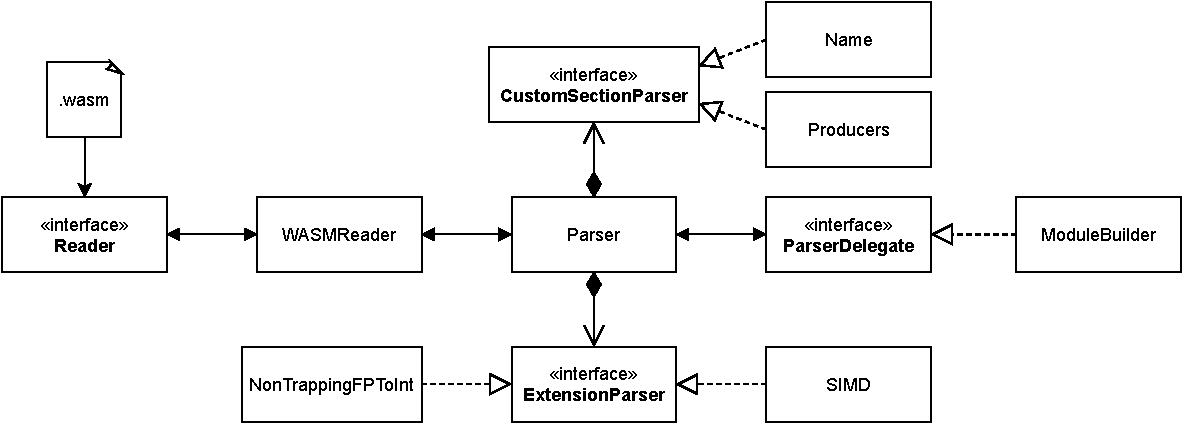
\includegraphics[width=\textwidth]{Images/sablewasm-parser.pdf}
  \caption{A illustration of SableWasm parser}
  \label{fig:sablewasm-parser}
\end{figure}

\paragraph{Byte-source Reader}
The byte-source reader consists of two parts, a byte-buffer reader and a WebAssmebly reader. The byte-buffer reader provides essential functionalities such as read and skips. Additionally, the byte-buffer reader also needs to support rewind and barrier. Any out of bound access, either beyond the barrier or byte stream exhausted, the byte-buffer reader will signal via exceptions. On the other hand, the WebAssembly reader provides a richer interface to the parser, such as decode LEB-128 encoded integers and parsing WebAssembly value types. The WebAssembly reader is also responsible for validating the result before passing it to the parser. In the case the result is invalid, the reader throws exceptions similar to the byte-buffer reader.

\paragraph{WebAssembly Parser}
WebAssembly parser is the kernel part of the parsing framework. As we discussed earlier in the chapter, one of the primary design goals of the framework is its extensibility. Hence, the SableWasm parser is modular and consists of three parts, parser core, custom section parser and instruction extension parser. The grammar for WebAssembly binary representation is quite simple, and hence, the parser core implements a simple top-down recursive descent parser with a single byte look-ahead.

\emph{Custom sections} are a special section defined in the WebAssembly standard. They are essentially a binary data chunk tagged with a string name. How to interpret the binary data is different from one to another. These custom sections can either be standardized by the community or defined specific to a toolchain. In this project, we implement two custom sections standardized by the WebAssembly working group, namely \emph{Name} section and \emph{Producer} section. The \emph{Name} section gives human-readable names to functions and their local variables that help program debugging. The specification does not require these names to be the same as the import or export names. There is no direct support for more detailed debug information encoding in WebAssembly, at the time of thesis writing. However, extensions are working on this problem, such as DWARF for WebAssembly \footnote{DWARF for WebAssembly: \url{https://yurydelendik.github.io/webassembly-dwarf/}}; on the other hand, the \emph{Producer} section is relatively simple. It only encodes the information about the toolchain that generates the module, such as the toolchain name and version. All custom section parsers in SableWasm derived from the base class \texttt{CustomSection}. The parser core will dispatch the binary chunk to search custom section parser based on the name tag. Each custom section parser manages its results and does not communicate to the parser delegate directly. Instruction extension parsers focus on another different aspect of the WebAssembly module.

In the background section, we have visited several extensions that merged to the WebAssembly specification. A quick reminder, WebAssembly extensions can insert or modify the instructions defined in the minimum-viable-product (MVP)  specification. The SableWasm WebAssembly parser employs instruction extension parsers to address this problem. When the parser intends to parse an instruction, it will iterate over all its instruction extension parsers in a chained manner. If the instruction opcode is not recognized by any registered instruction extension parser nor in the minimum-viable-product specification, the parser will signal the error by throwing an exception. 


\section{WebAssembly Bytecode Representation}

\section{WebAssembly Bytecode Validation}

\section{Performance Evaluation}